\chapter{The Sub-Problem Structure of Manipulation Tasks}
\label{chap:formulation}

In this chapter,
we lay out the structure of the manipulation planning problem
in detail.
We also outline our approach.

Definitely reference DRC Trials paper for planning vs. execution
time breakdown!

In Section~\ref{sec:subprobs:structure},
we describe the structure of these tasks.
In Section~\ref{sec:subprobs:related},
we discuss approaches in the literature
to handle this structure.
In Section~\ref{sec:subprobs:approach},
we descrive our approach.

\section{Scope}

Not handling feedback to high-level symbolic planner
(e.g. what failed and why?)
like hybrid planners do
(e.g. Plaku \& Kavraki, DARRT, HPN, etc).

Though our approach is in part complementary?

\section{Structure of Manipulaiton Tasks}
\label{sec:subprobs:structure}

We are motivated to solve motion planning problems for articulated robots.
In the simplest version of this problem,
the robot has a continuous configuration space $C$,
with some subset $C_{obs}$ in collision.
All feasible trajectories must then lie entirely in
$\mathcal{C}_{\mbox{\scriptsize free}} = C \setminus C_{obs}$.
In general, testing some configuration $q$ for membership in
$\mathcal{C}_{\mbox{\scriptsize free}}$
is an expensive operation.
A typical query asks for a trajectory $t: [0,1] \rightarrow Q$ between
a start set and a goal set (e.g. $t(0) \in Q_s$ and $t(1) \in Q_g$.
We defer discussion constraints until later.
We are focused on configuration spaces without dynamics.

{
\setlength{\offsetpage}{0.5in}
\begin{figure}
\begin{widepage}
\centering

   \begin{subfigure}[t]{0.19\linewidth}
      \centering
      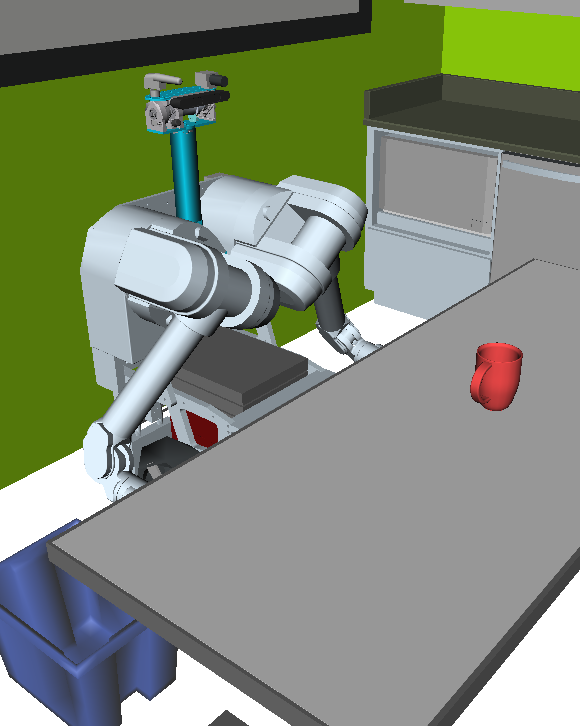
\includegraphics[width=\columnwidth]{figs/testherb-a.png}
      \caption{Start config}
   \end{subfigure}
   \begin{subfigure}[t]{0.19\linewidth}
      \centering
      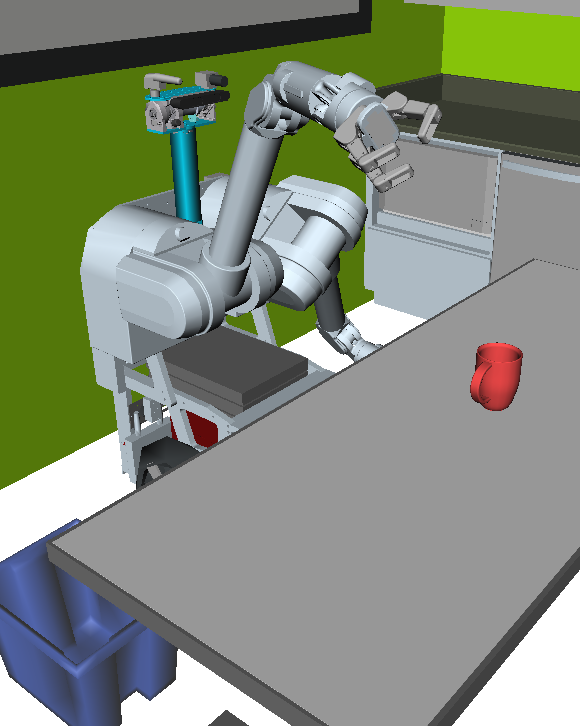
\includegraphics[width=\columnwidth]{figs/testherb-b.png}
      \caption{Step 1 in $X_1$}
   \end{subfigure}
   \begin{subfigure}[t]{0.19\linewidth}
      \centering
      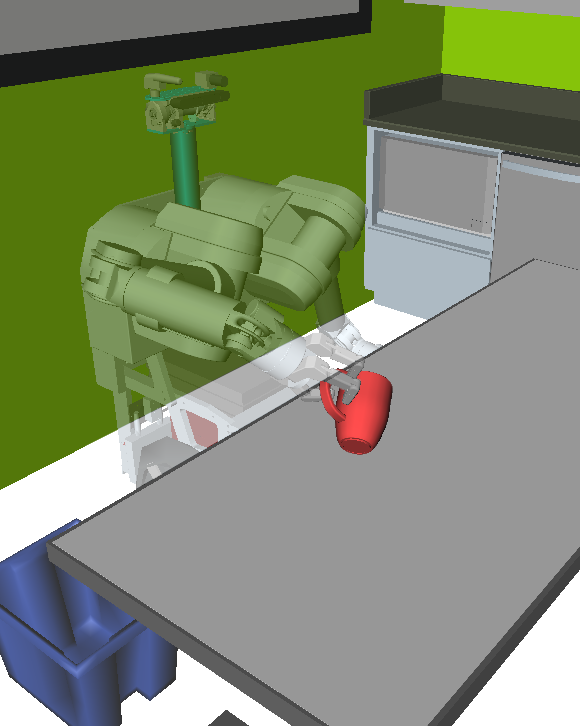
\includegraphics[width=\columnwidth]{figs/testherb-c.png}
      \caption{Step 2 in $X_2$}
   \end{subfigure}
   \begin{subfigure}[t]{0.19\linewidth}
      \centering
      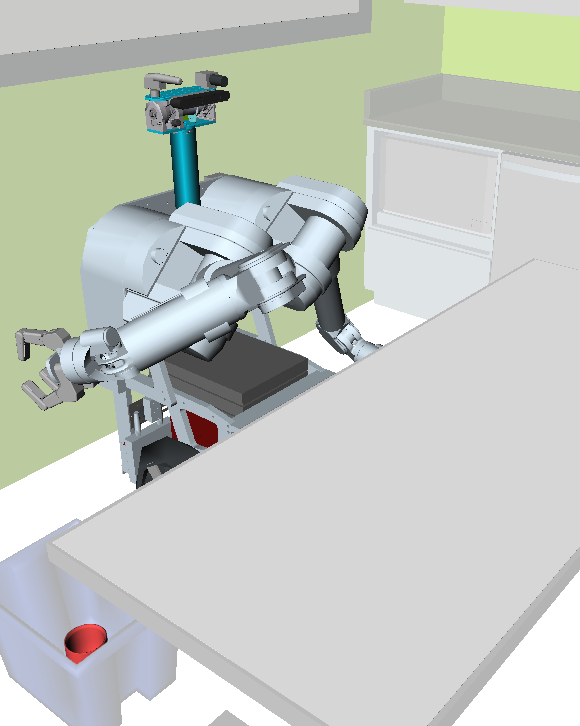
\includegraphics[width=\columnwidth]{figs/testherb-d.png}
      \caption{Step 3 in $X_3$}
   \end{subfigure}
   \begin{subfigure}[t]{0.19\linewidth}
      \centering
      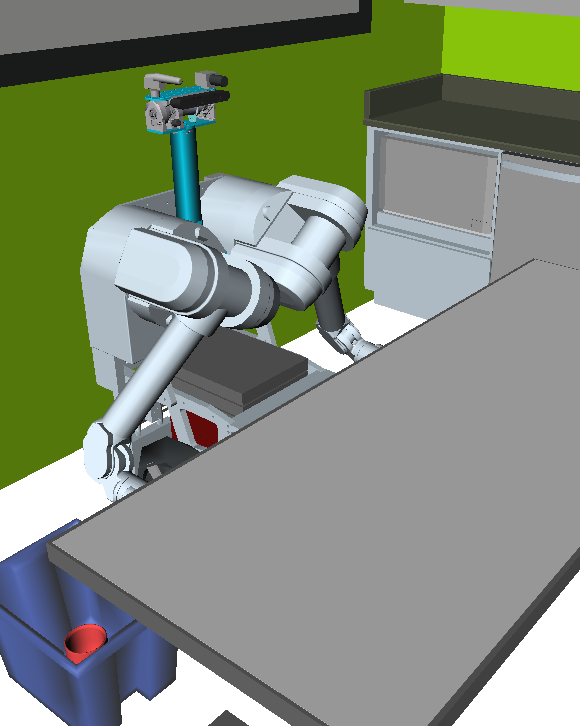
\includegraphics[width=\columnwidth]{figs/testherb-e.png}
      \caption{End config}
   \end{subfigure}

   \vspace{0.3cm}

   \begin{subfigure}[t]{\linewidth}
      \centering
      \includegraphics{build/diagram-multi-step}
      \caption{This thesis focuses on efficient geometric planning
         for manipulation tasks (the lower two levels here).
         Task planning can be performed by an autonomous
         symbolic planner,
         or guided by a human operator.}
   \end{subfigure}

   \caption{Diagram of multi-step planning framework.}
   \label{fig:diagram-multi-step}
\end{widepage}
\end{figure}
}

The manipulation problem has a particular structure,
which we discuss here.
See Figure~\ref{fig:diagram-multi-step}
for a diagram.

\subsection{Specification of Configuration-Space Interfaces
   and Constraints}

We are NOT solving the symbolic task planning problem.
Our pieces would be useable by such a planner,
including one which reasons about different orders.
But for the purpose of this thesis,
we'll basically assume that the sequence is given to us.

Complementary to symbolic planners
or from humans (e.g. the DRC \cite{dellin2014drc}).

For this proposal,
will only discuss seqential sub-plans,
but an intelligent meta-planner
can do non-sequential stuff too.

Not doing research here -- just need something that specifies
geometric goals.

From DRC Trials: Fixtures as a Common Language!

\section{Related Work}
\label{sec:subprobs:related}

How have others solved manipulation problems with sub-problem
structure?

Also, talk about planning in the now stuff
when discussing the scope of the thesis.

\subsection{DRC Trials Approach}

Talk a lot about the DRC approach.
It was slow, and it got stuck!

Copy-paste in from the ISER paper \cite{dellin2014drc}!

Used a bidirectional RRT.
Deep-dive into DRC Trials data analysis from ISER paper.
This will help really connect with all three challenges
identified in the introduction.

\subsection{Other Related Work}

We only talk here about related work
in the context of the sub-problems in manipulation problems.
Alternative approaches to solving each piece
(e.g. optimizers, etc)
are in Chapter~\ref{chap:graphs-in-continuous}.

Talk about subgoals in A* literature.

\section{Approach}
\label{sec:subprobs:approach}

Here we discuss how we address this sub-problem structure.
This serves as a more detailed outline of the remaining
thesis chapters.
We can go into a lot more detail about the relationships
between the chapters than we could in the intro.

Briefly discuss the higher-level planner.

Multi-step problem structure (lots of options at each step);
decomposition into a bunch of "local planner" like things.
We're essentially building a meta-graph.
Don't get stuck.

We talk a lot about the mapping
from continuous spaces to graphs in
Chapter~\ref{chap:graphs-in-continuous}.

For now, assume a prescribed order,
but we'll talk later about more complex meta-planning
approaches
in Chapter~\ref{chap:task-planning}
when we put it all together.

The bulk of the thesis ignores
interleaved planning execution,
but Chapter~\ref{chap:task-planning}
talks about it.

\subsection{When Does Our Approach Work?}

Sidd mentioned making a table of some kind
identifying what properties of problems are particularly
well-suited to our approach,
which I think is a great idea.

Some of this has to be bourne out through more experimentation.

\subsection{Root Sampling}

Do root sampling at the higher level
(to ensure consistency between the sub-planners).
(Can't rely on the sub-planners to generate their own starts/goals --
they must be synchronized.)

We talk briefly about learning good intermediate goals
in Section~\ref{subsec:learning-good-intermediate-roots}.

\subsection{Addressing Efficiency Within Steps}

The proposal is split into two complementary things,
guided by how slow collision checking is.

Chapters 3,4 focus WITHIN each step.
Make each step fast.

While there are many types of approaches for such queries
which we discuss in Section~\ref{sec:related-work},
one of the most common are graph search algorithms.

\subsection{Addressing Efficiency Between Steps}

Chapters 5,6 focus BETWEEN steps.
Exploit structure between steps (Chapter~\ref{chap:multi-set}).
Single-query vs. multi-query.

\subsection{Addressing Robustness of Full Planner}

CMR, etc.

\subsection{Other Stuff}

Other stuff to touch on
(mostly with pointers to later chapters):
\begin{itemize}
\item Dealing with constraints
\item Dealing with dual-arm stuff
\item Dealing with optimizers (run afterwards!)
   Most solution paths will be unexecuted, so optimize later!
\end{itemize}
